\chapter{Variations et extremums de fonctions}

\section{Notions de croissance et de décroissance}

\subsection{Définitions}

\begin{defin}[Sens de variation]
	Soit $f$ une fonction définie sur un intervalle $I$.
	\begin{itemize}
		\item $f$ est \textbf{croissante} sur $I$ si pour tous réels $a$ et $b$ de $I$ tels que $a < b$, on a :
		      \[
			      f(a) \le f(b)
		      \]
		\item $f$ est \textbf{décroissante} sur $I$ si pour tous réels $a$ et $b$ de $I$ tels que $a < b$, on a :
		      \[
			      f(a) \ge f(b)
		      \]
	\end{itemize}
\end{defin}

\begin{ex}
	\nline
	\begin{itemize}
		\item \textbf{Illustration de la croissance sur $]0 \,;\, +\infty[$ :}

					      Pour la fonction $f: x \mapsto x^2$, si l'on choisit $a = 2$ et $b = 3$ (on a $a < b$), on constate que :
					      \[ f(2) = 2^2 =4\quad\text{ et }\quad f(3) = 3^2 \]

					      On observe que $f(2) < f(3)$ : l'ordre est conservé sur ces deux valeurs.

					      Cet exemple illustre le comportement de la fonction, mais pour \textbf{démontrer} qu'elle est croissante sur $]0 \,;\, +\infty[$, il faut le vérifier pour \textbf{tous} réels $a$ et $b$ tels que $0 < a < b$.

		\item \textbf{Illustration de la décroissance sur $]0 \,;\, +\infty[$ :}

		      Pour la fonction $g: x \mapsto \dfrac{1}{x}$, si l'on choisit $a = 2$ et $b = 4$ (on a $a < b$), on constate que :

		      \[
			      g(2) =\frac{1}{2}= 0{,}5\quad \text{ et }\quad g(4) = \frac{1}{4}=0{,}25
		      \]

		      On observe que $g(2) > g(4)$ : l'ordre est renversé pour ces deux valeurs.
	\end{itemize}
\end{ex}

\begin{rem}
	\nline
	\begin{itemize}
		\item Une fonction \textbf{croissante} \textbf{conserve l'ordre} des nombres et de leurs images.
		\item Une fonction \textbf{décroissante} \textbf{renverse l'ordre} des nombres et de leurs images.
		\item On parle de croissance ou décroissance \textbf{strictes} lorsque les inégalités sont strictes ($f(a) < f(b)$ ou $f(a) > f(b)$).
		\item Dire qu'une fonction est \textbf{monotone} sur un intervalle signifie qu'elle est soit uniquement croissante, soit uniquement décroissante sur cet intervalle.
	\end{itemize}
\end{rem}

\newpage

\begin{prop}[Interprétation graphique]
	\nline
	\begin{itemize}
		\item La courbe représentative d'une fonction croissante \textbf{monte} de la gauche vers la droite.
		\item La courbe représentative d'une fonction décroissante \textbf{descend} de la gauche vers la droite.
	\end{itemize}
	\begin{center}
		\begin{tikzpicture}[scale=0.9, >=Stealth]
			\begin{scope}
				\draw[->, thick] (-0.5,0) -- (4,0) node[right, font=\small] {$x$};
				\draw[->, thick] (0,-0.5) -- (0,3.5) node[above, font=\small] {$y$};
				\def\xa{0.8} \def\ya{0.75}
				\def\xb{3.2} \def\yb{2.55}
				\draw[thick, black, domain=0.2:3.8] plot (\x, {0.15*(\x+0.5)^2 + 0.5});
				\draw[dashed, gray] (\xa,0) node[below, black, font=\small] {$a$} -- (\xa,\ya) -- (0,\ya) node[left, black, font=\small] {$f(a)$};
				\draw[dashed, gray] (\xb,0) node[below, black, font=\small] {$b$} -- (\xb,\yb) -- (0,\yb) node[left, black, font=\small] {$f(b)$};
				\node[circle, fill=red!60!black, inner sep=1.5pt] at (\xa,\ya) {};
				\node[circle, fill=red!60!black, inner sep=1.5pt] at (\xb,\yb) {};
				\node[font=\small, black] at (1.75,-1) {$a < b \implies f(a) \le f(b)$};
			\end{scope}
			\begin{scope}[xshift=7cm]
				\draw[->, thick] (-0.5,0) -- (4,0) node[right, font=\small] {$x$};
				\draw[->, thick] (0,-0.5) -- (0,3.5) node[above, font=\small] {$y$};
				\def\xa{0.8} \def\ya{2.8465}
				\def\xb{3.2} \def\yb{1.06}
				\draw[thick, black, domain=0.2:3.8] plot (\x, {-0.15*(\x+0.5)^2 + 3.1});
				\draw[dashed, gray] (\xa,0) node[below, black, font=\small] {$a$} -- (\xa,\ya) -- (0,\ya) node[left, black, font=\small] {$f(a)$};
				\draw[dashed, gray] (\xb,0) node[below, black, font=\small] {$b$} -- (\xb,\yb) -- (0,\yb) node[left, black, font=\small] {$f(b)$};
				\node[circle, fill=red!60!black, inner sep=1.5pt] at (\xa,\ya) {};
				\node[circle, fill=red!60!black, inner sep=1.5pt] at (\xb,\yb) {};
				\node[font=\small, black] at (1.75,-1) {$a < b \implies f(a) \ge f(b)$};
			\end{scope}
		\end{tikzpicture}
	\end{center}
\end{prop}

\subsection{Extremums d'une fonction}

\begin{defin}[Maximum et Minimum]
	Soit $f$ une fonction définie sur un ensemble $D$.
	\begin{itemize}
		\item $f$ admet un \textbf{maximum} $M$ sur $D$, atteint en $a$, si pour tout $x \in D$ :
		      \[
			      f(x) \le M \quad \text{avec} \quad f(a) = M
		      \]
		\item $f$ admet un \textbf{minimum} $m$ sur $D$, atteint en $b$, si pour tout $x \in D$ :
		      \[
			      f(x) \ge m \quad \text{avec} \quad f(b) = m
		      \]
	\end{itemize}
	Un maximum ou un minimum est appelé un \textbf{extremum}.
\end{defin}

\begin{rem}
	Graphiquement, le maximum correspond à l'ordonnée du point le plus haut de la courbe, et le minimum à l'ordonnée du point le plus bas.
\end{rem}

\section{Tableau de variations}

\begin{defin}[Tableau de variations]
	Étudier les variations d'une fonction consiste à déterminer les intervalles sur lesquels elle est croissante ou décroissante. On résume ces comportements dans un \textbf{tableau de variations}.
\end{defin}

\begin{ex}
	Soit $f$ une fonction définie sur l'intervalle $[-3 \,;\, 6]$.
	
	On sait que :
	\begin{itemize}
		\item $f$ est strictement croissante sur $[-3 \,;\, 1]$, avec $f(-3) = -2$ et $f(1) = 5$ ;
		\item $f$ est strictement décroissante sur $[1 \,;\, 6]$, avec $f(6) = 0$.
	\end{itemize}

	On résume l'ensemble de ces informations dans le tableau de variations suivant :

	\begin{center}
		\begin{tikzpicture}
			\tkzTabInit[lgt=1.5, espcl=3]{$x$ / 0.75, $f(x)$ / 2}{$-3$, $1$, $6$}
			\tkzTabVar{-/ $-2$, +/ $5$, -/ $0$}
		\end{tikzpicture}
	\end{center}
\end{ex}

\newpage

\begin{methode}[Dresser un tableau de variations à partir d'une courbe]
	On considère la fonction $f$ représentée graphiquement ci-dessous :
	\begin{center}
		\begin{tikzpicture}[scale=0.8]
			\draw[very thin, gray!40] (-5.5,-4.5) grid (7.5,4.5);
			\draw[-{Stealth}, black] (-5.5,0) -- (7.5,0) node[above] {$x$};
			\draw[-{Stealth}, black] (0,-4.5) -- (0,4.5) node[right] {$y$};
			\foreach \x in {-5,...,-1,1,2,...,7} \node[below, font=\small, black] at (\x,0) {\x};
			\foreach \y in {-4,...,-1,1,2,...,4} \node[left, font=\small, black] at (0,\y) {\y};
			\draw[very thick] plot[smooth] coordinates {(-5,-2)(-4,-4)(-3,-2)(-2,0)(0,3.5)(1,2)(2,1.5)(3,0.8)(5,-3)(7,1)};
			\filldraw[red] (-5,-2) circle (0.1);
			\filldraw[red] (-4,-4) circle (0.1);
			\filldraw[red] (0,3.5) circle (0.1);
			\filldraw[red] (5,-3) circle (0.1);
			\filldraw[red] (7,1) circle (0.1);
			\node[black, font=\large] at (2,2) {$\mathcal{C}_f$};
		\end{tikzpicture}
	\end{center}

	\begin{enumerate}
		\item Préciser l'ensemble de définition $D_f$ de $f$.
		\item Décrire les variations de $f$.
		\item Identifier les extremums de $f$ sur son ensemble de définition.
		\item Dresser le tableau de variations synthétique.
		\item Comparer, en justifiant par les variations de $f$, les nombres $f(1)$ et $f(4)$.
		\item Peut-on comparer $f(-2)$ et $f(2)$ uniquement à l'aide des variations de $f$ ?
	\end{enumerate}

	\begin{correction}
		\nline
		\begin{enumerate}
			\item La fonction est définie pour $x \in [-5 \,;\, 7]$.
			\item $f$ est décroissante sur $[-5 \,;\, -4]$ et $[0 \,;\, 5]$, puis croissante sur $[-4 \,;\, 0]$ et $[5 \,;\, 7]$.
			\item Le maximum de $f$ est $3{,}5$ (atteint en $x = 0$) et son minimum est $-4$ (atteint en $x = -4$).
			\item Tableau de variations :
			      \ms
			      \begin{center}
				      \begin{tikzpicture}
					      \tkzTabInit[lgt=1.5, espcl=2]{$x$ / 0.75, $f(x)$ / 2}{$-5$, $-4$, $0$, $5$, $7$}
					      \tkzTabVar{+/ $-2$, -/ $-4$, +/ $3{,}5$, -/ $-3$, +/ $1$}
				      \end{tikzpicture}
			      \end{center}
		    \item Les nombres $1$ et $4$ appartiennent tous les deux à l'intervalle $[0 \,;\, 5]$ sur lequel la fonction $f$ est strictement décroissante.

		           Comme $1 < 4$, la fonction $f$ renverse l'ordre, d'où $f(1) > f(4)$.
		    \item Non. Le nombre $-2$ appartient à l'intervalle $[-4 \,;\, 0]$ où $f$ est croissante, tandis que $2$ appartient à l'intervalle $[0 \,;\, 5]$ où $f$ est décroissante.

				Les variations de la fonction sur deux intervalles distincts ne permettent pas de comparer leurs images directes sans information supplémentaire.
		\end{enumerate}
	\end{correction}
\end{methode}
